\subsection{Electron Fake Rate}

We summarize the electron fake rate measurements in this appendix section. We use the same
fakeable object definition described in reference \cite{HWW2011}. Also an analogous trigger
selection is used.

\subsubsection{Trigger Bias}
Due to the evolving trigger menu, the requirements on the electron legs of the electron muon
triggers and the double electron triggers are different for different run ranges. Essentially
three different levels of requirements are imposed:


\begin{itemize}
  \item HLT Electron (HLT\_Ele8),
  \item CaloIdL CaloIsoVL (HLT\_Ele8\_CaloIdL\_CaloIsoVL),
  \item CaloIdT TrkIdVL CaloIsoVL TrkIsoVL (HLT\_Ele8\_CaloIdT\_TrkIdVL\_CaloIsoVL\_TrkIsoVL).
\end{itemize}

In Figure \ref{fig:ele_fr_triggerBiasCheck} we verify that the different trigger requirements do not result in a bias of the
electron fake rate, in the nominal fake rate measurement sample with a leading jet $p_{T}$ cut of $35$ \GeV\ and the
sample with a leading jet $p_{T}$ cut of $15$ \GeV\ where statistical uncertainties are much smaller. As a result 
we can use all fake rate trigger samples and perform a combined fake rate measurement which can be applied to 
all final states.

\begin{figure}[!htbp]
\begin{center}
\subfigure[]{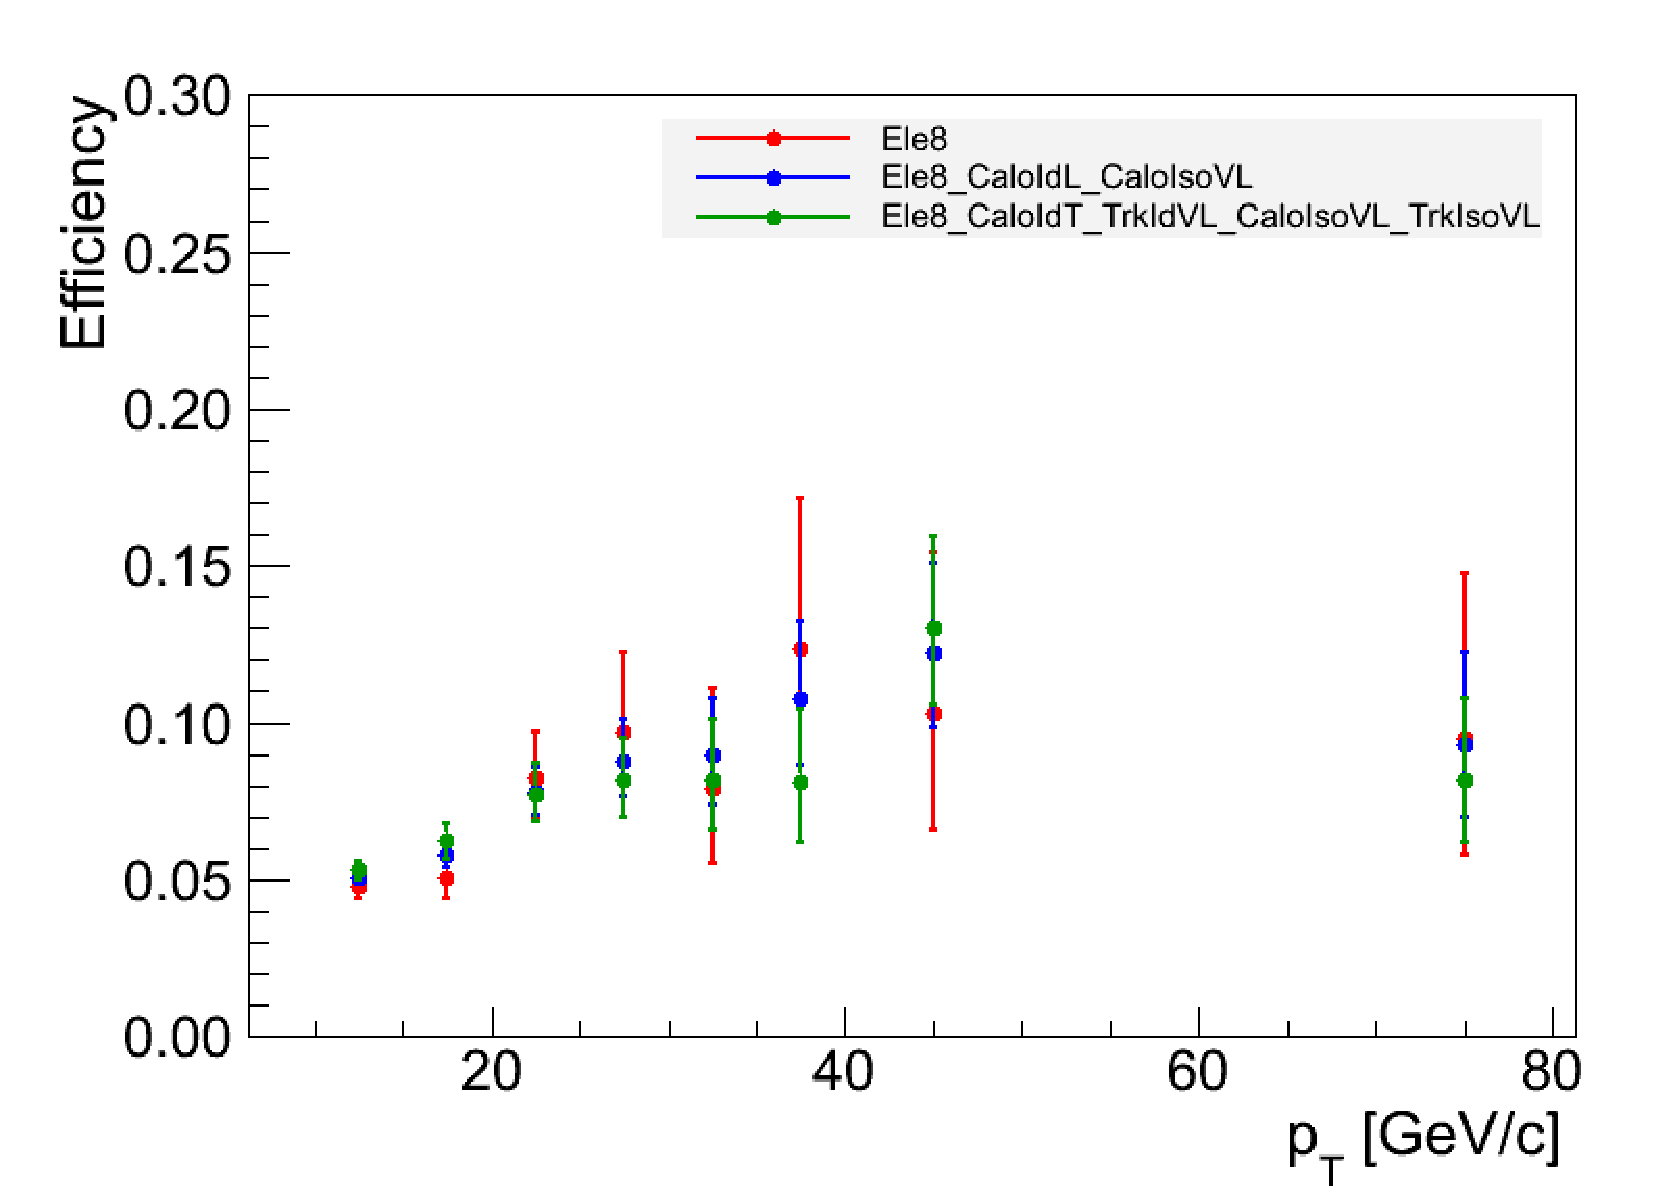
\includegraphics[width=0.45\textwidth]{figures/ElectronFakeRate_JetPt15_VsTriggers.pdf}}
\subfigure[]{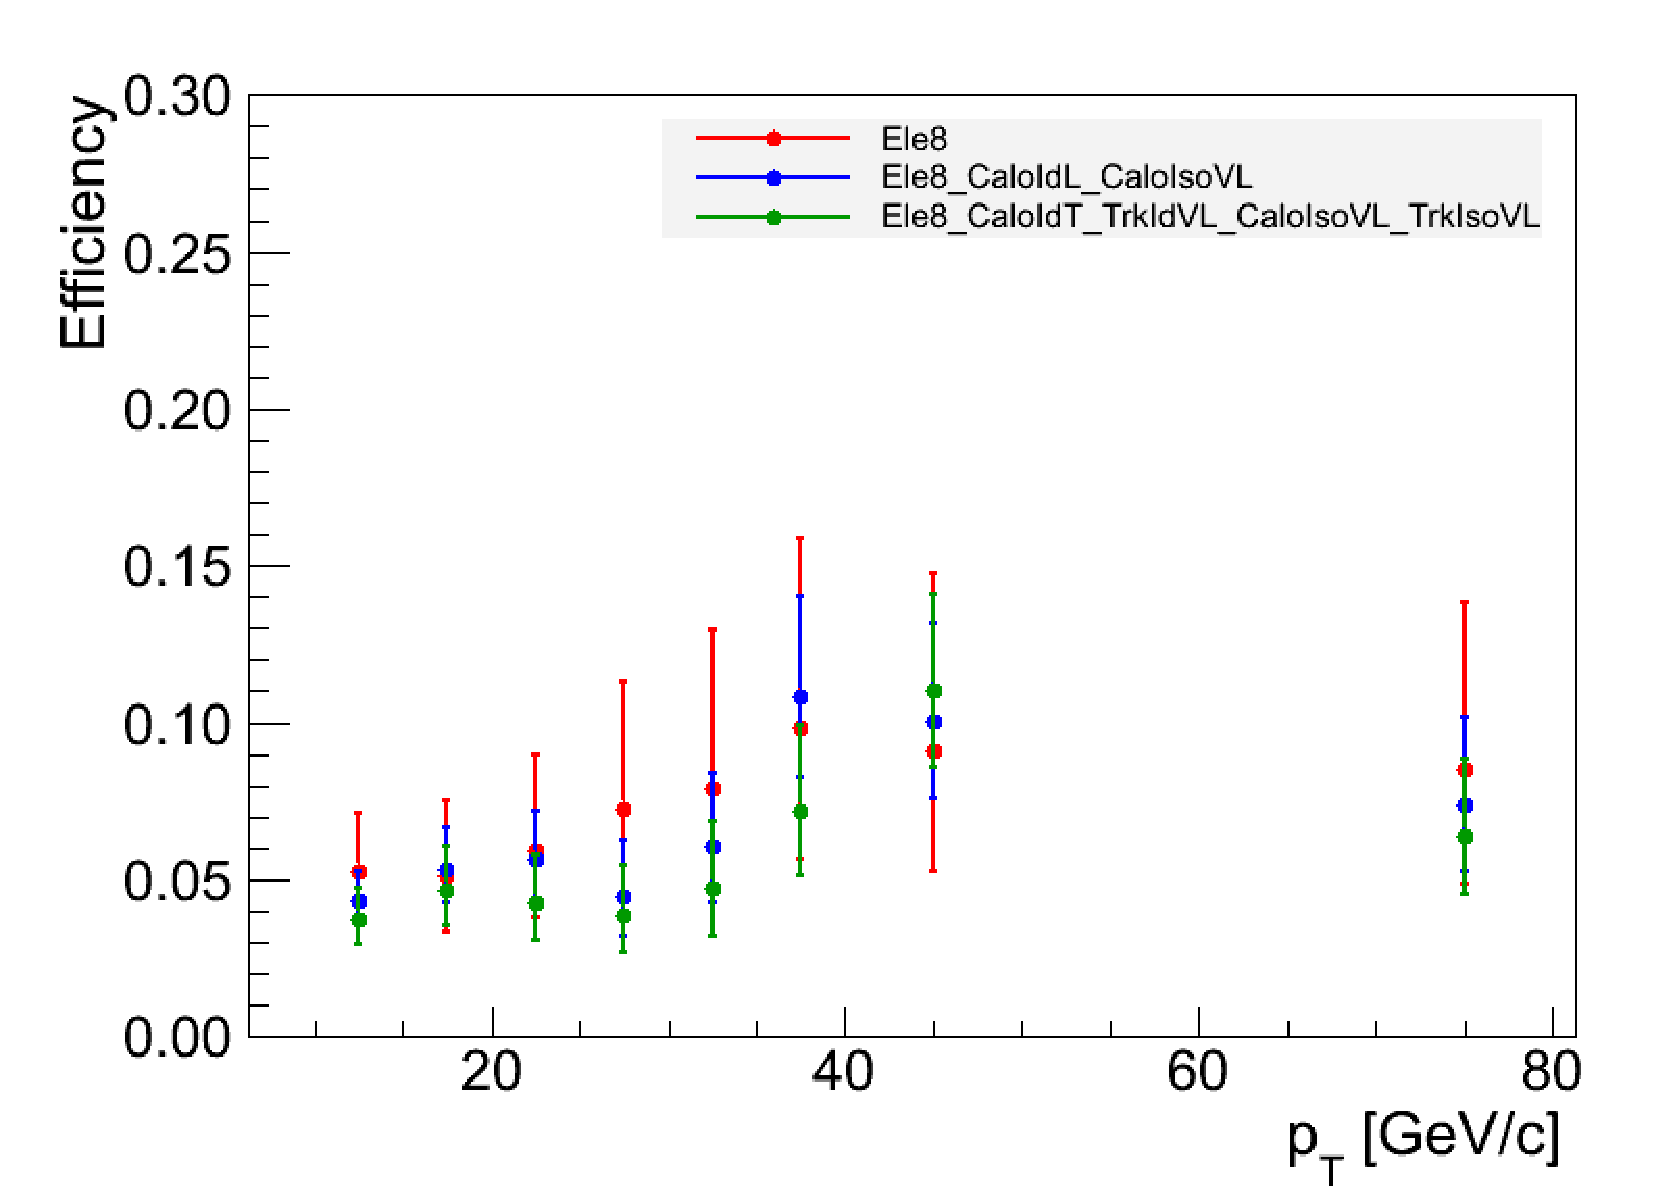
\includegraphics[width=0.45\textwidth]{figures/ElectronFakeRate_JetPt35_VsTriggers.pdf}}
\caption{Electron fake rates as a function for $p_{T}$ for different trigger samples.}
\label{fig:ele_fr_triggerBiasCheck}
\end{center}
\end{figure}



\subsubsection{Electron Fake Rate Results}

The electron fake rates measured for the full 2011 data requiring the leading jet $p_{T}$ to be 
larger than $35$ GeV are shown in Figure \ref{fig:ele_fr_Full2011} as a function of the $p_{T}$ 
and $\eta$ of the electron. The fake rates are tabulated in the 
$p_{T}$ and $\eta$ bins used to perform the background estimate in Table~\ref{tab:ele_fr_Full2011}.


\begin{figure}[!htbp]
\begin{center}
\subfigure[$p_{T}$]{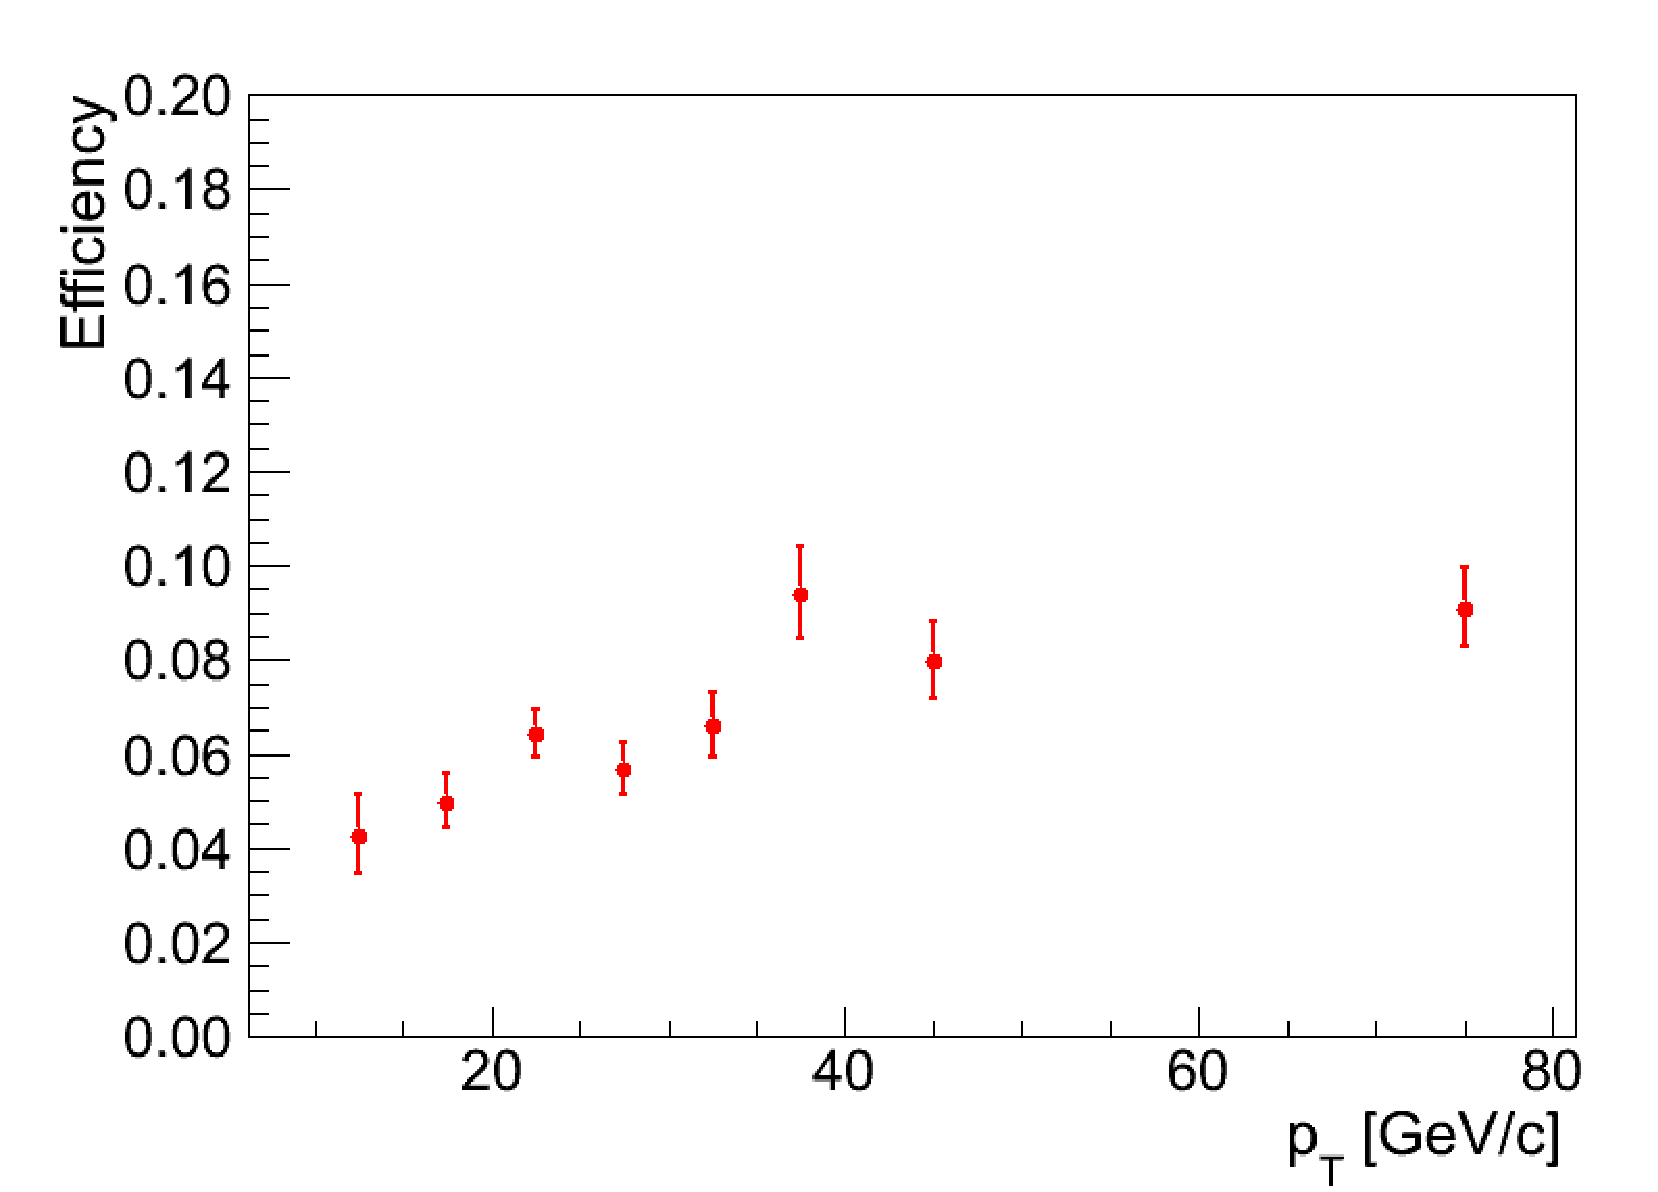
\includegraphics[width=0.45\textwidth]{figures/ElectronFakeRate_Pt.pdf}}
\subfigure[$\eta$]{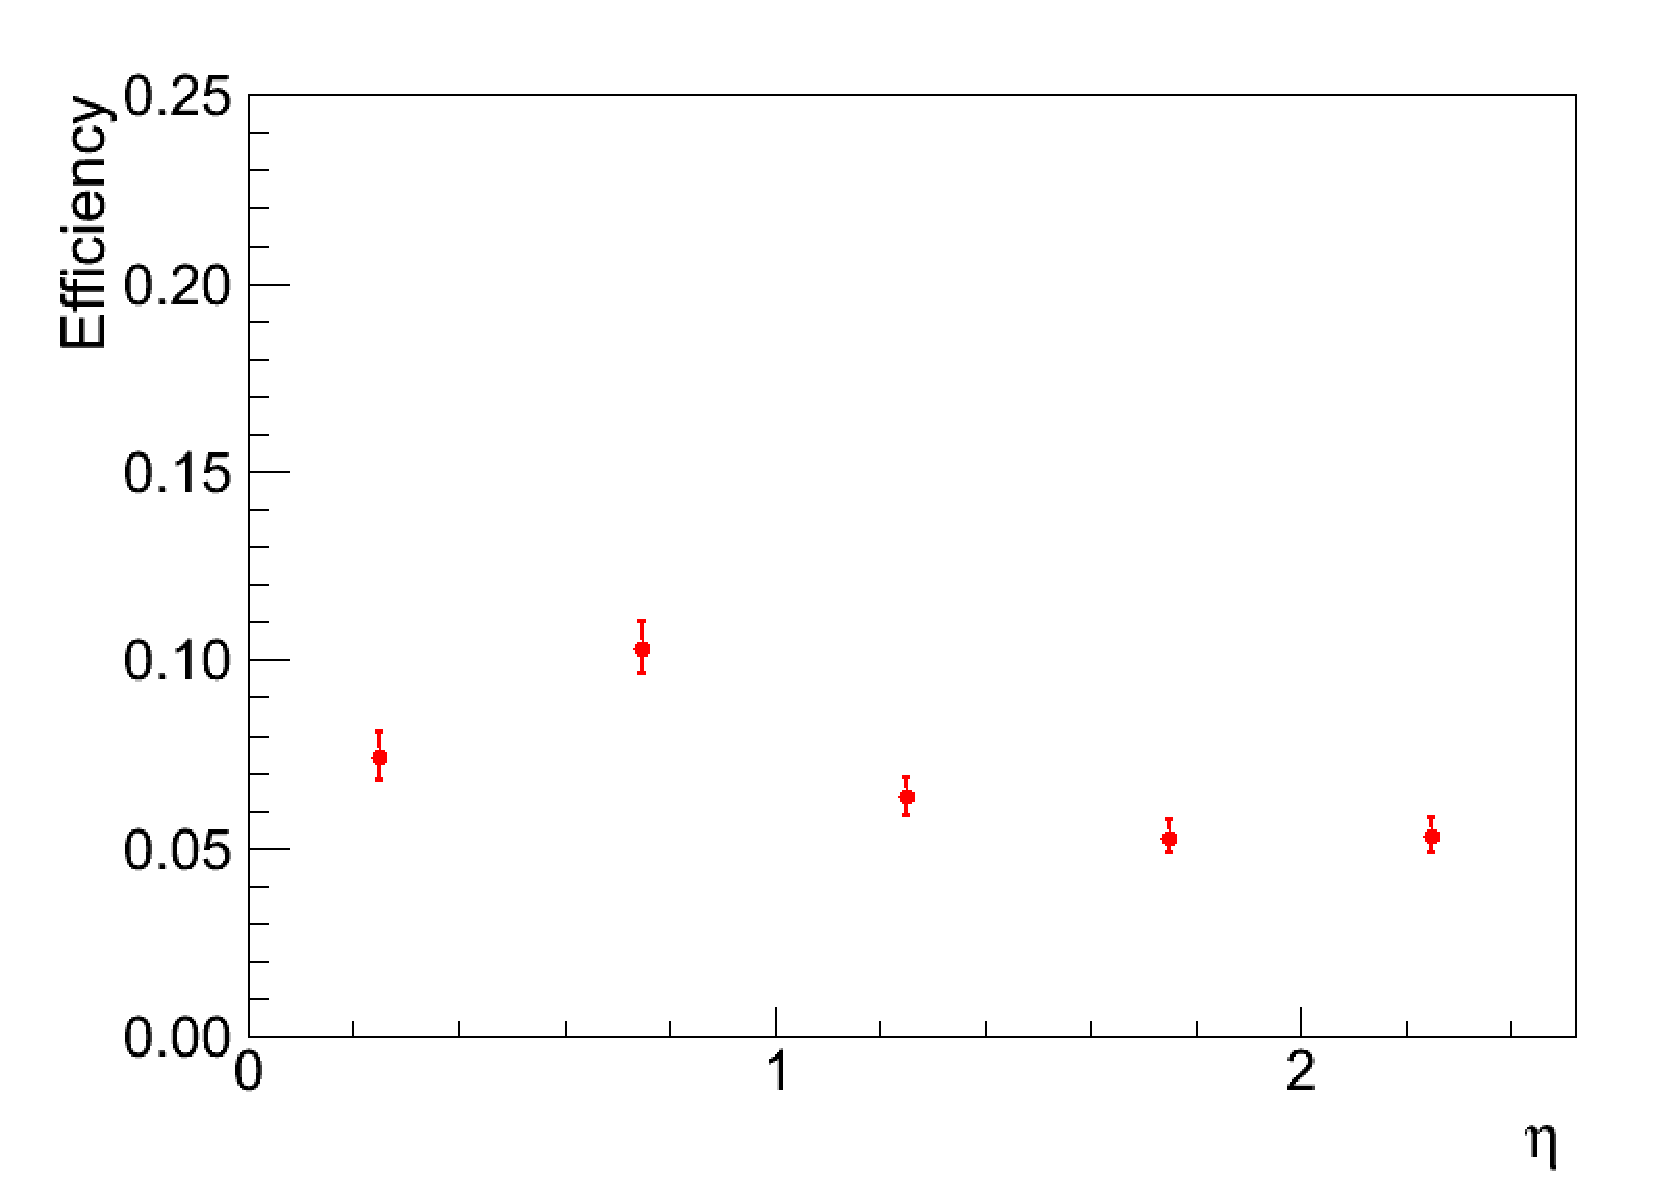
\includegraphics[width=0.45\textwidth]{figures/ElectronFakeRate_Eta.pdf}}
\caption{Electron fake rates as a function for $p_{T}$ and $\eta$ for the full 2011 dataset.}
\label{fig:ele_fr_Full2011}
\end{center}
\end{figure}


\begin{table}[!htbp]
\begin{center}
\begin{tabular}{|c|c|c|c|c|c|}

\hline
                       &        $0<\eta<1.0$      &        $1.0<\eta<1.479$  &        $1.479<\eta<2.0$  &        $2.0<\eta<2.5$     \\
\hline
    $10 < p_{T} <= 15$ &        $0.070 +/- 0.010$ &        $0.037 +/- 0.008$ &        $0.023 +/- 0.007$ &        $0.030 +/- 0.009$  \\ 
 \hline
    $15 < p_{T} <= 20$ &        $0.075 +/- 0.009$ &        $0.043 +/- 0.008$ &        $0.016 +/- 0.005$ &        $0.038 +/- 0.009$  \\ 
 \hline
    $20 < p_{T} <= 25$ &        $0.088 +/- 0.009$ &        $0.064 +/- 0.009$ &        $0.049 +/- 0.008$ &        $0.042 +/- 0.007$  \\ 
 \hline
    $25 < p_{T} <= 30$ &        $0.080 +/- 0.009$ &        $0.054 +/- 0.010$ &        $0.035 +/- 0.007$ &        $0.066 +/- 0.010$  \\ 
 \hline
    $30 < p_{T} <= 35$ &        $0.078 +/- 0.011$ &        $0.085 +/- 0.014$ &        $0.073 +/- 0.012$ &        $0.051 +/- 0.010$  \\ 
 \hline

\end{tabular}
\caption{Electron fake rate in $\eta$-$p_T$ using the full 2011 data.
Uncertainties are statistical only. A combination of the {\bf Ele8\_CaloIdL\_CaloIsoVL}, {\bf Ele17\_CaloIdL\_CaloIsoVL}, 
{\bf Ele8\_CaloIdL\_CaloIsoVL\_Jet40}, and 
{\bf HLT\_Ele8\_CaloIdT\_TrkIdVL\_CaloIsoVL\_TrkIsoVL} triggers are used, with a $p_{T}$ threshold on the leading jet in
the event of $35$ GeV. }
\label{tab:ele_fr_Full2011}
\end{center}
\end{table}


\subsubsection{Pileup Dependence}

Due to the effect of energy from pileup interactions on the electron isolation, there is a small 
dependence of the fake rate on the number of reconstructed primary vertices shown in 
Figure \ref{fig:ele_fr_PileupDependence}.


\begin{figure}[!htbp]
\begin{center}
\subfigure[Number of Reconstructed Primary Vertices]{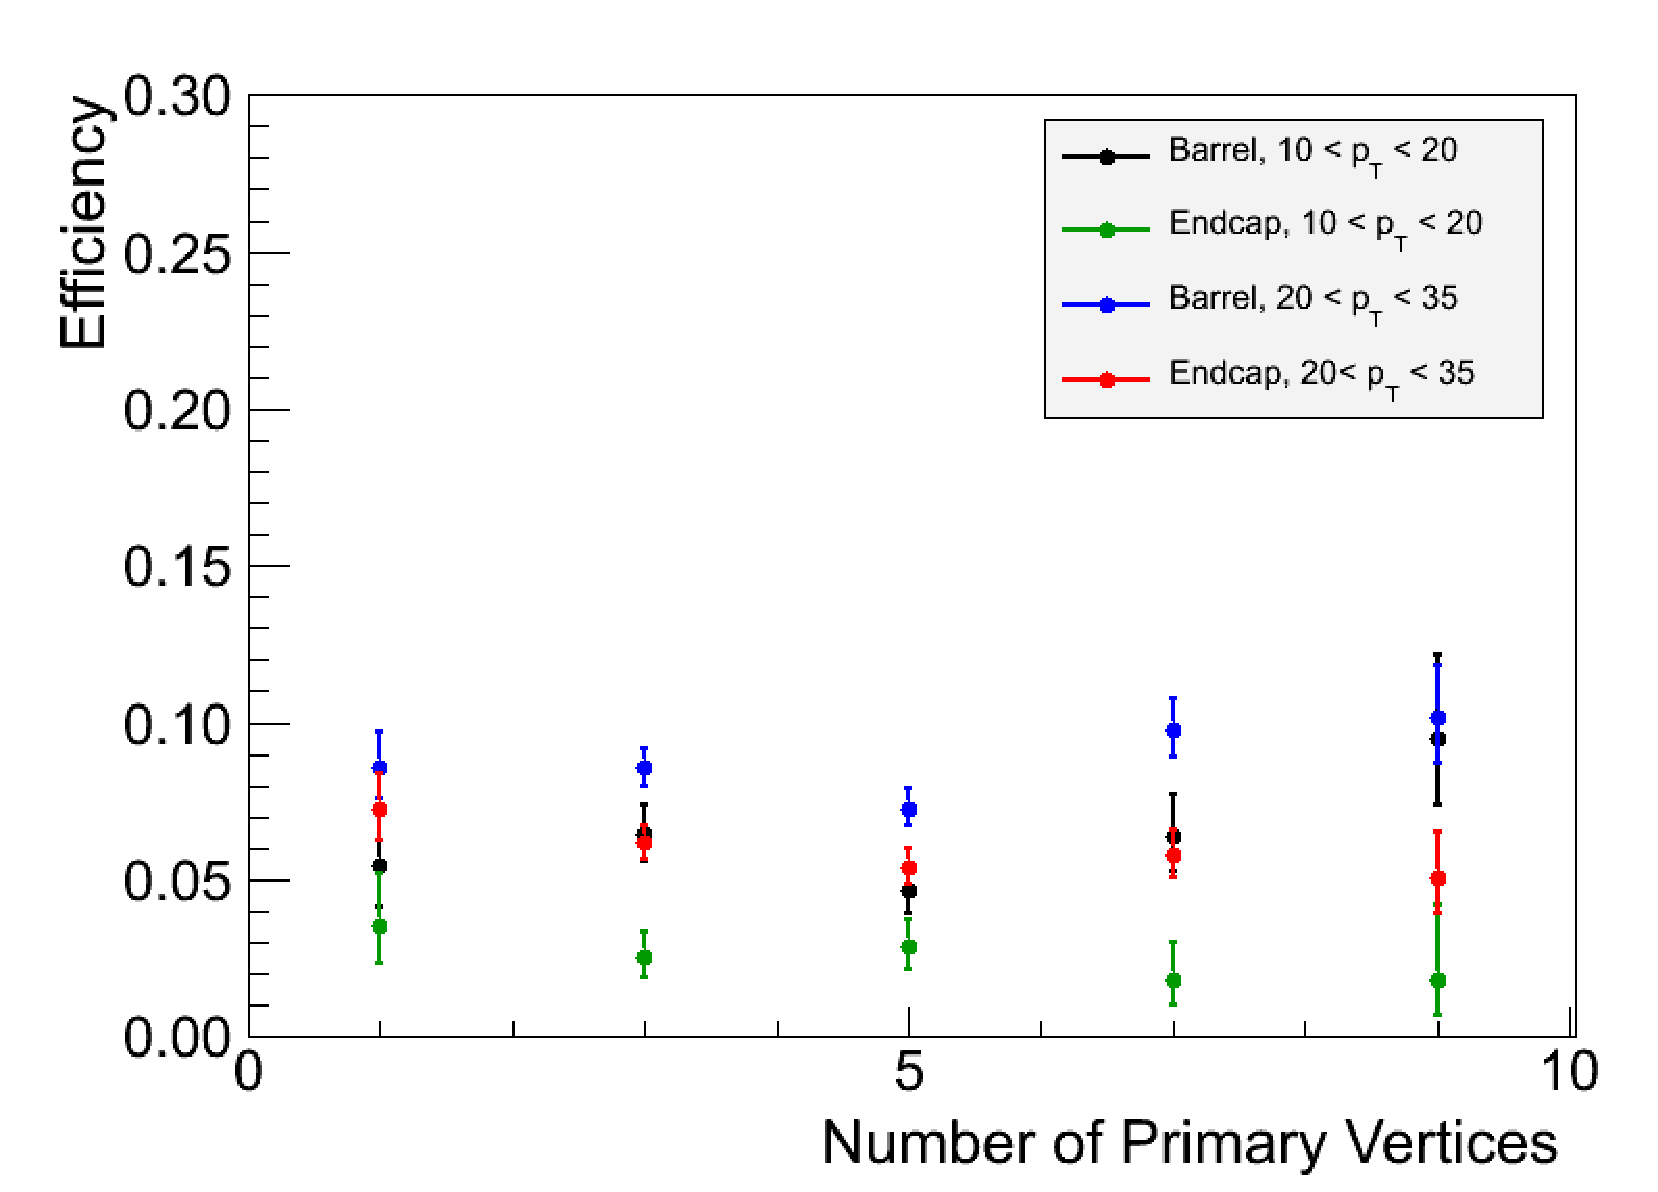
\includegraphics[width=0.45\textwidth]{figures/ElectronFakeRate_NVtx.pdf}}
\subfigure[Pileup Energy Density ($\rho$)]{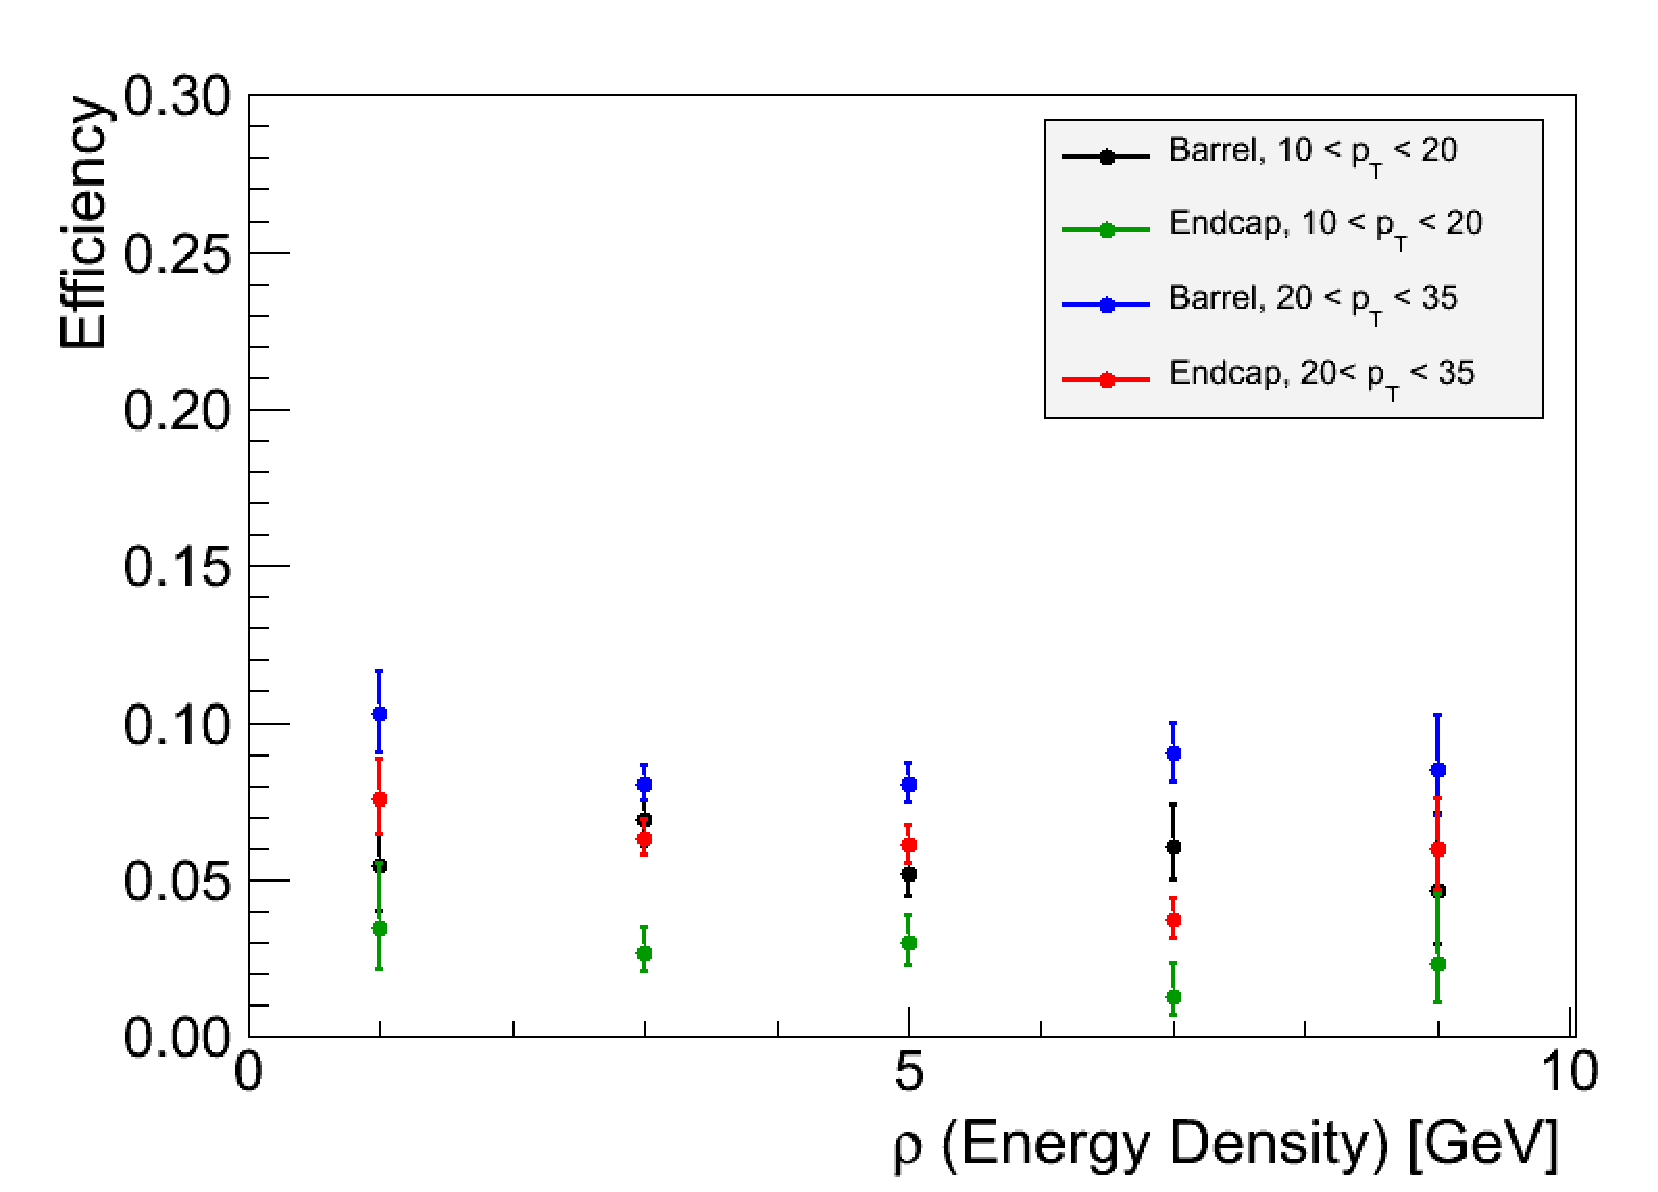
\includegraphics[width=0.45\textwidth]{figures/ElectronFakeRate_Rho.pdf}}
\caption{Electron fake rates as a function of the number of reconstructed primary vertices (a) 
and the pileup energy density (b) in four different $p_{T}$ and $\eta$ bins.}
\label{fig:ele_fr_PileupDependence}
\end{center}
\end{figure}


\begin{table}[!htbp]
\begin{center}
\begin{tabular}{|c|c|c|c|c|c|}

\hline
                       &        $0<\eta<1.0$      &        $1.0<\eta<1.479$  &        $1.479<\eta<2.0$  &        $2.0<\eta<2.5$     \\
\hline
    $10 < p_{T} <= 15$ &        $0.091 +/- 0.035$ &        $0.016 +/- 0.016$ &        $0.016 +/- 0.016$ &        $0.067 +/- 0.037$  \\ 
 \hline
    $15 < p_{T} <= 20$ &        $0.055 +/- 0.024$ &        $0.043 +/- 0.025$ &        $0.033 +/- 0.023$ &        $0.050 +/- 0.028$  \\ 
 \hline
    $20 < p_{T} <= 25$ &        $0.091 +/- 0.026$ &        $0.051 +/- 0.025$ &        $0.049 +/- 0.024$ &        $0.000 +/- 0.000$  \\ 
 \hline
    $25 < p_{T} <= 30$ &        $0.094 +/- 0.030$ &        $0.127 +/- 0.045$ &        $0.025 +/- 0.017$ &        $0.042 +/- 0.024$  \\ 
 \hline
    $30 < p_{T} <= 35$ &        $0.096 +/- 0.034$ &        $0.018 +/- 0.017$ &        $0.141 +/- 0.043$ &        $0.083 +/- 0.040$  \\ 
 \hline

\end{tabular}
\caption{Electron fake rate in $\eta$-$p_T$ using the full 2011 data in events with 1 or 2 reconstructed primary vertices.
Uncertainties are statistical only. A combination of the {\bf Ele8\_CaloIdL\_CaloIsoVL}, {\bf Ele17\_CaloIdL\_CaloIsoVL}, 
{\bf Ele8\_CaloIdL\_CaloIsoVL\_Jet40}, and 
{\bf HLT\_Ele8\_CaloIdT\_TrkIdVL\_CaloIsoVL\_TrkIsoVL} triggers are used, with a $p_{T}$ threshold on the leading jet in
the event of $35$ GeV. }
\label{tab:ele_fr_Full2011_low}
\end{center}
\end{table}

\begin{table}[!htbp]
\begin{center}
\begin{tabular}{|c|c|c|c|c|c|}

\hline
                       &        $0<\eta<1.0$      &        $1.0<\eta<1.479$  &        $1.479<\eta<2.0$  &        $2.0<\eta<2.5$     \\
\hline
    $10 < p_{T} <= 15$ &        $0.071 +/- 0.014$ &        $0.027 +/- 0.010$ &        $0.023 +/- 0.010$ &        $0.031 +/- 0.012$  \\ 
 \hline
    $15 < p_{T} <= 20$ &        $0.073 +/- 0.012$ &        $0.046 +/- 0.012$ &        $0.007 +/- 0.005$ &        $0.048 +/- 0.014$  \\ 
 \hline
    $20 < p_{T} <= 25$ &        $0.065 +/- 0.011$ &        $0.079 +/- 0.014$ &        $0.047 +/- 0.011$ &        $0.048 +/- 0.011$  \\ 
 \hline
    $25 < p_{T} <= 30$ &        $0.085 +/- 0.014$ &        $0.043 +/- 0.013$ &        $0.029 +/- 0.009$ &        $0.079 +/- 0.015$  \\ 
 \hline
    $30 < p_{T} <= 35$ &        $0.058 +/- 0.013$ &        $0.109 +/- 0.023$ &        $0.067 +/- 0.016$ &        $0.055 +/- 0.016$  \\ 
 \hline

\end{tabular}
\caption{Electron fake rate in $\eta$-$p_T$ using the full 2011 data in events with 3, 4, or 5 reconstructed primary vertices.
Uncertainties are statistical only. A combination of the {\bf Ele8\_CaloIdL\_CaloIsoVL}, {\bf Ele17\_CaloIdL\_CaloIsoVL}, 
{\bf Ele8\_CaloIdL\_CaloIsoVL\_Jet40}, and 
{\bf HLT\_Ele8\_CaloIdT\_TrkIdVL\_CaloIsoVL\_TrkIsoVL} triggers are used, with a $p_{T}$ threshold on the leading jet in
the event of $35$ GeV. }
\label{tab:ele_fr_Full2011_med}
\end{center}
\end{table}

\begin{table}[!htbp]
\begin{center}
\begin{tabular}{|c|c|c|c|c|c|}

\hline
                       &        $0<\eta<1.0$      &        $1.0<\eta<1.479$  &        $1.479<\eta<2.0$  &        $2.0<\eta<2.5$     \\
\hline
    $10 < p_{T} <= 15$ &        $0.063 +/- 0.015$ &        $0.059 +/- 0.017$ &        $0.027 +/- 0.012$ &        $0.017 +/- 0.012$  \\ 
 \hline
    $15 < p_{T} <= 20$ &        $0.086 +/- 0.015$ &        $0.037 +/- 0.013$ &        $0.020 +/- 0.010$ &        $0.021 +/- 0.012$  \\ 
 \hline
    $20 < p_{T} <= 25$ &        $0.112 +/- 0.016$ &        $0.045 +/- 0.013$ &        $0.049 +/- 0.013$ &        $0.048 +/- 0.013$  \\ 
 \hline
    $25 < p_{T} <= 30$ &        $0.068 +/- 0.014$ &        $0.051 +/- 0.016$ &        $0.043 +/- 0.013$ &        $0.060 +/- 0.016$  \\ 
 \hline
    $30 < p_{T} <= 35$ &        $0.097 +/- 0.020$ &        $0.085 +/- 0.023$ &        $0.058 +/- 0.018$ &        $0.034 +/- 0.014$  \\ 
 \hline

\end{tabular}
\caption{Electron fake rate in $\eta$-$p_T$ using the full 2011 data in events with 6 or more reconstructed primary vertices.
Uncertainties are statistical only. A combination of the {\bf Ele8\_CaloIdL\_CaloIsoVL}, {\bf Ele17\_CaloIdL\_CaloIsoVL}, 
{\bf Ele8\_CaloIdL\_CaloIsoVL\_Jet40}, and 
{\bf HLT\_Ele8\_CaloIdT\_TrkIdVL\_CaloIsoVL\_TrkIsoVL} triggers are used, with a $p_{T}$ threshold on the leading jet in
the event of $35$ GeV. }
\label{tab:ele_fr_Full2011_high}
\end{center}
\end{table}



